\documentclass[12pt]{article}

\usepackage[utf8]{inputenc}
\usepackage[russian]{babel}
\usepackage{graphicx}
\usepackage{indentfirst}
\usepackage{booktabs}


\graphicspath{{pic/}}

\begin{document}

\begin{center}
	\LARGE 
	\textbf{Практическое занятие 2}\\
	ОПЕРАЦИИ С ВЕКТОРАМИ И МАТРИЦАМИ В СИСТЕМЕ MATLAB\\
\end{center}

\begin{flushright}
	\large
	Игнашов Иван\\
	Вариант 8\\
\end{flushright}

\newpage

 \section*{1. Цель работы}
Изучение реализации средствами системы MATLAB основных операций с векторами и матрицами.
\subsection*{Порядок работы:}
\begin{enumerate}
	\item Ввод с клавиатуры векторов и матриц.\\
		Ввести:
		\begin{itemize}
			\item произвольную вектор-строку (v), размерность 2;
			\item произвольный вектор-столбец (w), размерность 2;
			\item произвольную матрицу (m), размерности 2×2.
		\end{itemize}
	\item Генерация матриц специального вида.\\
		Создать:
		\begin{itemize}
			\item матрицу с нулевыми элементами (m0), размерности 2×2;
			\item матрицу с единичными элементами(m1), размерности 2×2;
			\item матрицу с элементами, имеющими случайные значения(mr), размерности 2×2;
			\item матрицу с единичными диагональными элементами(me), размерности 2×2.
		\end{itemize}
	\item Вычисление матрицы M по формуле\\
		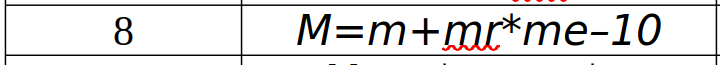
\includegraphics[width=0.5\linewidth]{formula.png}
	\item Изучение функций обработки данных:
		\begin{itemize}
			\item определение числа строк и столбцов матрицы M;
			\item определение максимального элемента матрицы M;
			\item определение минимального элемента матрицы M;
			\item суммирование элементов матрицы M;
			\item перемножение элементов матрицы M.
		\end{itemize}
\end{enumerate}

 \section*{2. Описание ввода с клавиатуры векторов и матриц}%
 
\begin{figure}[!h]
	\centering
	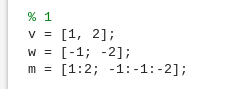
\includegraphics[width=0.4\linewidth]{1_matrix_set.png}
	\caption{Ввод векторов и матриц}
\end{figure}

Матрицы \textit{v} и \textit{w} - одномерные вектора, положение данных в которых различаются символом разделения - `;` или `,` \\

При заполнении матрицы \textit{m} отрицательными числами использовался шаг $-1$ чтобы заполнить строку от максимального к минимальному
 
  \section*{3. Описание команд генерации матриц специального вида}%
  
\begin{figure}[!h]
	\centering
	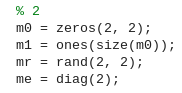
\includegraphics[width=0.4\linewidth]{2_spec_matrix_set.png}
	\caption{Генерация матриц специального вида}
\end{figure}

Для генерации диагональной матрицы \textit{me} требовалось указать только одно измерение т.к. диагональная матрица обязательно генерируется квадратной

\begin{figure}
  \section*{4. Описание основных функций обработки данных}%
\end{figure}

  
\begin{figure}[!h]
	\centering
	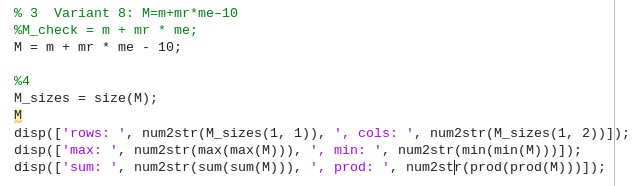
\includegraphics[width=\linewidth]{3_data_manipulating.png}
	\caption{Генерация и обработка матрицы \textit{M}}
\end{figure}

Для нахождения количества строк и столбцов матрицы \textit{M} использовалось то, что метод \textit{size(A)} возвращает одномерный вектор: первый элемент - количество строк; второй - количество столбцов\\

Так как методы \textit{max(A)}, \textit{min(A)}, \textit{sum(A)}, \textit{prod(A)} работают по столбцам, приходится вызывать их 2 раза, чтобы свести двумерную матрицу к скаляру.

\begin{figure}[!h]
	\centering
	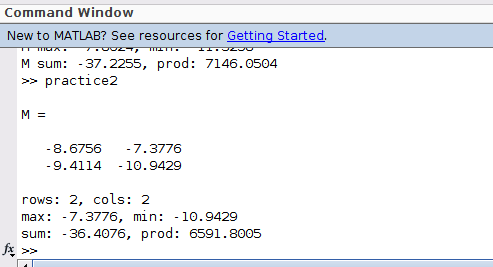
\includegraphics[width=0.75\linewidth]{output.png}
	\caption{Пример вывода данных}
\end{figure}

\end{document}